\documentclass[a4paper, 11pt]{report}
\usepackage{cs_thesis}
\usepackage[pdftex]{graphicx}
\usepackage[utf8]{inputenc}
\usepackage{amsmath}
\usepackage{url}
\usepackage{biblatex}
\usepackage{dtklogos}
\usepackage{listings}
\usepackage{color}
\usepackage[tocflat]{tocstyle}
\usetocstyle{standard}

\usepackage{blindtext}
\makeatletter
\renewcommand\tableofcontents{
  \hfill\textbf{\Large\contentsname}\hfill\null\par
  \@mkboth{\MakeUppercase\contentsname}{\MakeUppercase\contentsname}%
  \@starttoc{toc}
}
\makeatother

\renewcommand{\UrlFont}{\small\tt}
\makeatletter
\def\footnoterule{\kern-8\p@
  \hrule \@height 1pt \@width 6in \kern 7.6\p@}
\renewcommand{\thempfootnote}{\arabic{mpfootnote}}
\makeatother

\lstset{language=C++,
  basicstyle=\ttfamily,
  keywordstyle=\color{blue}\ttfamily,
  stringstyle=\color{red}\ttfamily,
  commentstyle=\color{green}\ttfamily,
  morecomment=[l][\color{magenta}]{\#}
}

\lstset{language=C++,
  keywordstyle=\color{blue},
  stringstyle=\color{red},
  commentstyle=\color{green},
  morecomment=[l][\color{magenta}]{\#}
}

\title{The iCub Humanoid Robot}
\author{Semih Onay}
\program{Computer Science}
\supervisor{Associated Professor Elena Battini Sönmez}


\begin{document}
  \pagenumbering{Roman}
  \makecstitle
  \tableofcontents
  \listoffigures
  
  \begin{symabbreviations}
    \sym{\textbf{YARP}}{Yet Another Robot Platform}
    \sym{}{} 
    \sym{DA}{Description of abbreviation}
  \end{symabbreviations}
  
{\tiny}\chapter{ABSTRACT}
Robot are evolving to the edge of the our knowledge. The software and hardware 
produced for them are disappears without leaving any signs. Exploring how to 
make robots are stable and long-lasting, without yielding our ability of 
changing sensors, hardwares and networks. Advancing over two fronts, software 
and hardware. For some time, we have been developing and using the YARP robot 
software architecture, which helps 
organize communication between sensors, processors, and actuators so that 
loose coupling is encouraged, making gradual system evolution much easier. YARP 
includes a model of communication that is transport-neutral, so that data 
flow is decoupled from the details of underlying networks and protocols in use. 
Importantly for the long term, YARP is designed to play well with other 
architectures.\linebreak Device drivers written for YARP can be ripped out and 
used without any “middleware.” On the network, basic interoperation is possible 
with a few lines of code in any language with a socket library, and maximally 
efficient interoperation can be achieved by following documented protocols. 
These features are not normally the first things that end-users look for when 
starting a project, but they are crucial for longevity.
We emphasize the strategic utility of the Free Software social contract to 
software development for small communities with idiosyncratic requirements. 
We also work to expand our community by releasing the design of our ICub 
humanoid under a free and open license, and funding development using this 
platform.
  
{\tiny}\chapter{ÖZET}

{\tiny}\chapter{INTRODUCTION}
  
The iCub is a humanoid robot that developed at Istituto Italiano di Tecnologia 
(IIT) as part of European project RobotCub and later adopted by more 
than 20 laboratories arround the world. It has 53 motors that can move the head,
arms and hands, midriff, and legs.It can see and hear, it has the sense of 
proprioception\footnote{Body configuration and movement using 
accelerometers and gyroscopes}. It’s designed to aid studies of human cognition 
and artificial 
intelligence. Project members developed computer simulator to experiment new 
techniques.
\par Computer simulations are getting important in area robotics 
area.Simulations may not provide real complexity of the physical world and 
not reliable as real dynamics. The simulator of iCub is an easy way to test 
new algorithms and methods instead of dealing with complex configuration of 
iCub hardware. The simulator is designed to be accurate as real world 
psychics and dynamics. Development is based on directly from first prototype 
of simulation environment Webots.\footnote{Webots : 
https://www.cyberbotics.com}It was 
expensive and had limited 
access to source code which made hard to modify source code in order to add 
some functionalties.Then iCub simulation created. Simulation environment uses 
\linebreak to simulate body 
movement and collision detection algorithms to measure psychical interaction 
with the world.ODE\footnote{Open Dynamics Engine : http://www.ode.org} is used 
in wide range of 
projects like GAZEBO\footnote{GAZEBO : http://gazebosim.org}. ODE is an open 
source physics engine forauthoring tools, computer games,etc.It uses 
OpenGL\footnote{Open Graphics Library : https://www.opengl.org} renderer and it 
has some disadvantages due to limitation of OpenGL engine computation 
efficiency on complex structures. iCub simulation is using OpenGL directly via 
SDL\footnote{Simple DirectMedia Layer : https://www.libsdl.org} which 
helps to render complex robot movements and com- putation efficient simulation 
observations. Simulator is free and available to anyone who interested in 
robotics and learning about basics of robotics.

{\tiny}\chapter{LITERATURE REVIEW}
Development of simulator is described by abstraction of parts to handle complex 
instructions more precisely and efficient. Some other external software 
libraries are used to reduce required time to animate given parts of robots 
body from parameters. Abstractions made it easy to implement new 
methods,algorithms into a simulation environment. Understanding of these 
libraries are the key of creating new interfaces and methods to robot in 
virtual world.
Action primitives are pre-defined inside a simulation environment to extend 
capability of creating new interfaces to virtual simulation world and can be 
changed or taught as different languages which helps to extend knowledge about  
languages.

{\tiny}\chapter{METHODOLOGY}
  \subsection{The YARP Arcitechture}
The computer simulation model of the iCub robot. Simulator allows to 
create realistic scenarios in where robot can interact with a virtual world and 
physical limitations and interactions that occur between the virtual world is 
simulated using open source library which is \cite{ODE} (Open Dynamics Engine) 
to provide accurate simulation of body dynamics.
\begin{figure}[h!]
  \centering
  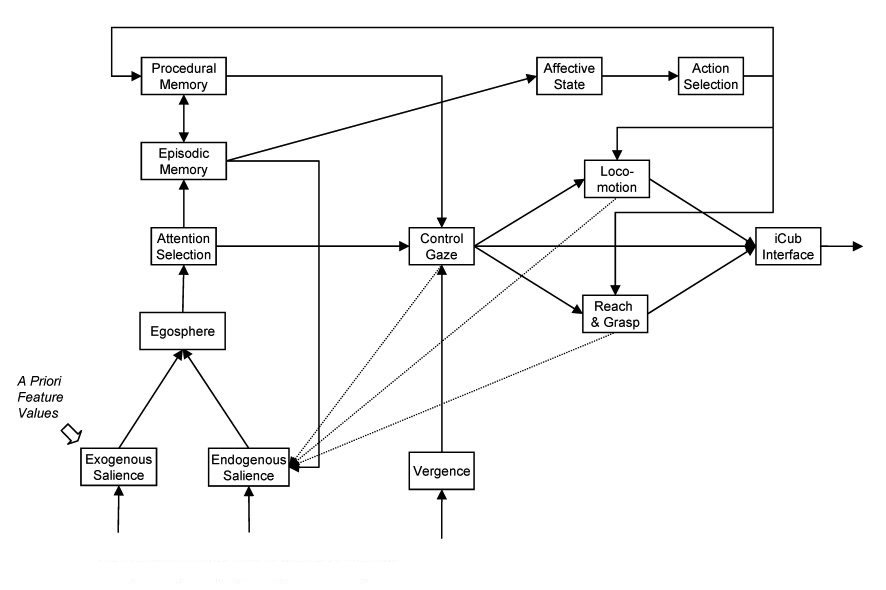
\includegraphics[width=1.0\linewidth]{cognitive_architecture}
  \caption{Cognitive Architecture of iCub}
  \label{fig:cognitive_architecture}
\end{figure}
Top of the \cite{YARP}. It is a set of open source 
libraries that supports modularity by using abstraction method in softwares 
to handle common difficulties in robotics area which are know as modularity 
algorithms, hardware interfaces and OS platforms.To deal with OS 
spesific builds,requires to use cross-platform build tools such as \cite{CMake} 
and \cite{ACE}. YARP is providing platform independence.First abstraction can 
be described as a protocols. Main YARP protocol manages interprocess 
communications in operating systems. It can deliver process messages of any 
size across the network by using different protocols.
\newpage
Second abstraction is about hardware communications.The method is to define 
interface for class of devices to fold native coded APIs.Changes in hardwares 
requires changes in API calls via linking suitable libraries to encapsulate 
hardware dependency problems. These two abstraction combined to use remote 
device drives where that can be accessed across the network like a parallel 
processing.
The purpose of YARP ports are to move data from threads to threads over the 
processes.Flow of the data can be configured and observed from command-line 
at real time. Port can receive or send data from any other port.Connections 
between ports can be modified easily with using different protocols such as 
TCP(Transmission Control Protocol) and UDP(User Datagram Protocol).The choice 
of protocol is depends on quality of message transmission or response 
time.Using TCP is for reliability and UDP is for speed with effect on 
unreliable transmissions.\linebreak

\begin{figure}[h!]
  \centering
  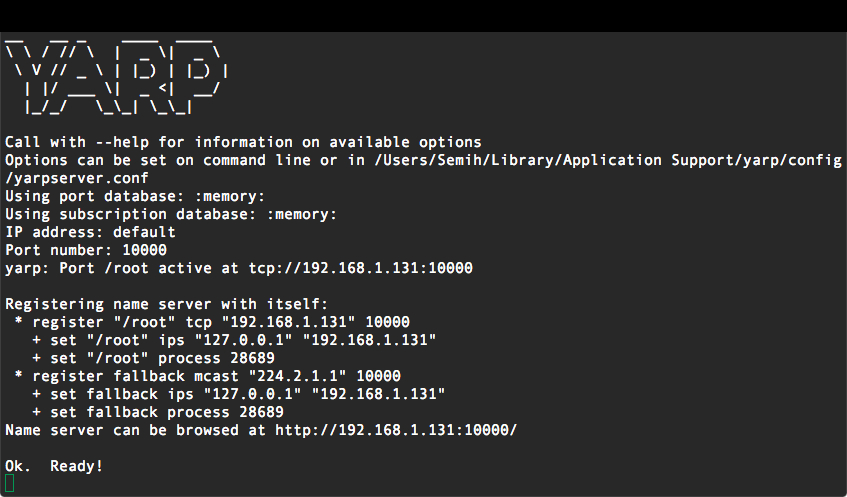
\includegraphics[width=1.0\linewidth]{yarp}
  \caption{YARP Command Line Interface}
  \label{fig:yarp}
\end{figure}
\subsection{The iCub Cognitive Architecture}
The design and realization of any cognitive architecture is a long-term 
project. The iCub cognitive architecture is no different. Inevitably, the 
realization happens in stages. In what follows, we describe a cognitive 
architecture which follows a signif- icant subset of the roadmap guidelines to 
a greater or lesser extent. The goal of this preliminary cognitive architecture 
is to integrate some of the phylogenetic capabili- ties identified in Chap. 6 
in a way that is meaningful for both neurophysiology and developmental 
psychology. In other words, the current goal is to build a minimal but faithful 
functioning system as a proof of principle. Sect. 7.3 discusses the degree to 
which each guideline has been followed and Chap. 8 considers the challenges 
posed by a complete implementation of the roadmap guidelines.
{\tiny}\begin{figure}[h!]
  \centering
  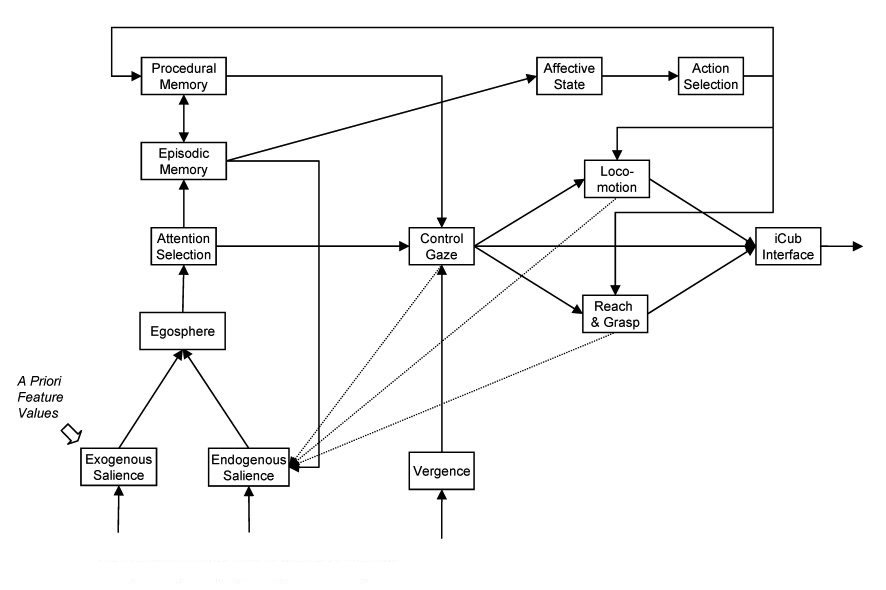
\includegraphics[width=1.0\linewidth]{cognitive_architecture}
  \caption{Cognitive Architecture of iCub}
  \label{fig:cognitive_architecture}
\end{figure}
The basis of the main conclusions, decided to research on some capabilities. 
Gaze control, reaching, and locomotion constitute the initial simple 
goal-directed actions. Episodic and procedural memories are 
included to effect a simplified version of internal simulation in order to 
provide capabilities for prediction and reconstruction, as well as generative 
model construction boot- strapped by learned affordances.
In addition, motivations encapsulated in the system’s affective state are made 
explicit so that they address curiosity and experimentation, both explorative 
mo- tives, triggered by exogenous and endogenous factors, respectively. This 
distinction between the exogenous and the endogenous is reflected by the need 
to include an attention system to incorporate both factors.
\newpage
\subsection{iCub Simulation Environment}
\begin{figure}[h!]
  \centering
  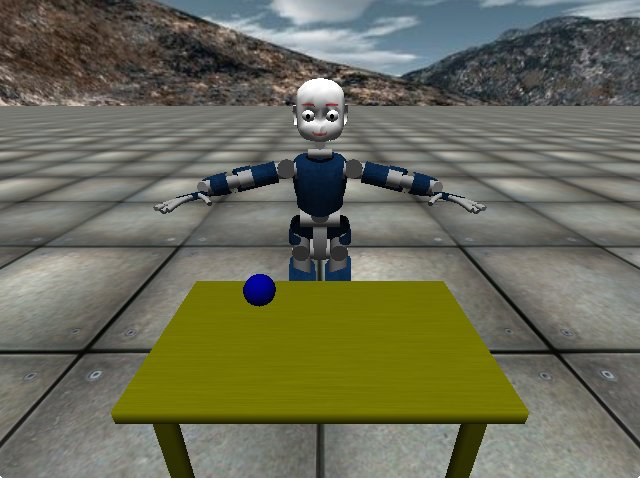
\includegraphics[width=1.0\linewidth]{sim}
  \caption{iCub Simulation Environment}
  \label{fig:icub}
  \end{figure}
\subsection{Mechanics of iCub}
\cite{David Vernon, The iCub}The kinematic specifications of the body of the 
iCub 
including the definition 
of the number of DOF and their actual locations as well as the actual size of 
the limbs and torso were based on ergonomic data and x-ray images.
The possibility of achieving certain motor tasks is favored by a suitable 
kinematics and, in particular, this translates into the determination of the 
range of movement and the number of controllable joints (where clearly 
replicating the human body in detail is impossible with current technology). 
Kinematics is also influenced by the overall size of the robot which was 
imposed a priori. The size is that of a 3.5 years old child (approximately 
100cm high). This size can be achieved with current technology. QRIO1 is an 
example of a robot of an even smaller size although with less degrees of 
freedom. In particular, our task specifications, especially manipulation, 
require at least the same  
  \begin{figure}[h!]
    \centering
    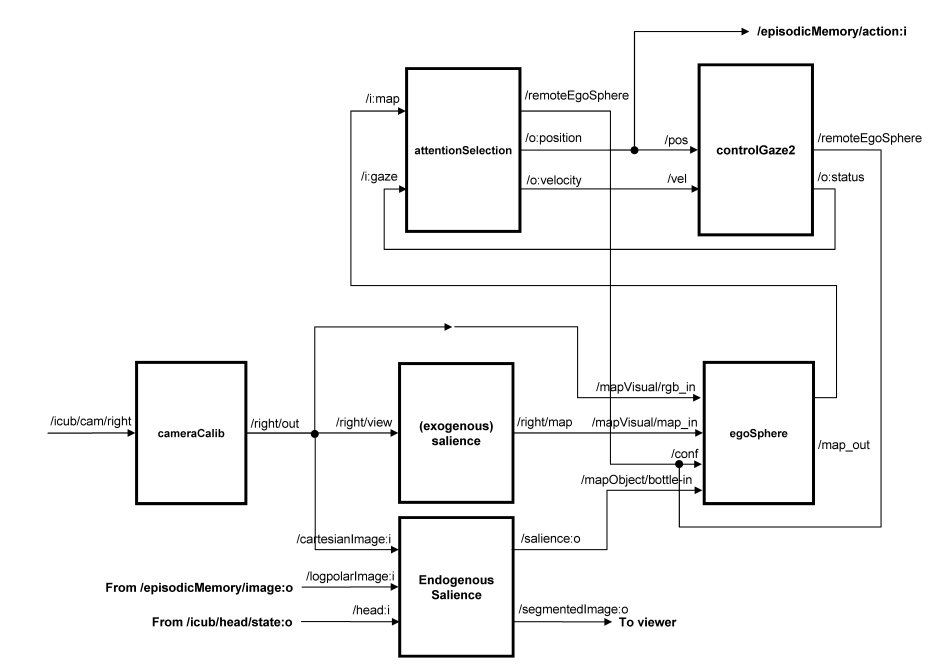
\includegraphics[width=0.9\linewidth]{cognitive_architecture_A}
    \caption{}
    \label{fig:cognitive_architecture_A}
  \end{figure} 

{\tiny}\chapter{RESULTS}

AŞSLFKASF
SF
S
F
ASF
sa
f
sf
s
F
sdf
asd
g
asdg

{\huge}\chapter{CONCULUSION}
Prediction, Reconstruction, and Action: Learning Affordances
Every action entails a prediction about how the perceptual world will change as 
a consequence of that action. This is the goal of the action and it is what 
differenti- ates an action from a simple movement or sequence of movements. 
Equivalently, every pair of perceptions is intrinsically linked or associated 
with an action. So, if we think of a perception-action-perception triplet of 
associations (Pi , A, Pj ), we can effect simple prediction, reconstruction (or 
explanation), and action as associative recall by presenting 
$(Pi,A,\tilde{a})$, 
$({\tilde{n}},A,Pj)$, or $(Pi,\tilde{a},Pj)$, respectively, to the 
iCub’s 
Procedural Memory and 
by 
associatively recalling the missing element. This triplet- based 
representation, is conceptually identical to the stand-alone iCub framework for 
learning object affordances [256, 257, 258]. What differs is the manner in 
which the association network is constructed. In the latter framework, learning 
is accom- plished by autonomous exploration using elementary actions that allow 
the iCub to experiment with its environment and to develop and understanding 
the relationships between actions, objects, and action outcomes, modelling 
these relationships using a Bayesian network. Affordances are represented by a 
triplet (O,A,E), where O is an object, A is an action performed on that object, 
and E is the effect of that action.  is the predictive aspect of 
%affordance; (O, E ) → A recognizes an action and aids planning; 
%(A,E) → O is object recognition and selection. One of our im- mediate goals is 
to integrate this affordance learning technique with the Procedural Memory and 
Episodic Memory components in the iCub cognitive architecture.
A significant problem remains, however. In the existing framework, the actions 
that the robot uses to experiment with and explore the object are assumed to 
ex- ist as predefined primitive manipulation movements, such as push, tap, and 
grasp. Clearly, we require a more flexible approach in which the action’s 
movements can be generated and adjusted adaptively as a consequence of the 
outcome of the action.
\subsection{Object Representation}
At present, there is no explicit concept of objecthood in the iCub cognitive 
archi- tecture in the sense of Guideline 15, and there are no visual processes 
which iden- tifies such objects. As we noted in the previous chapter, the 
implementation of this capability is far from trivial but, in principle, it 
doesn’t pose a major challenge us- ing conventional computer vision techniques 
based on motion segmentation and boundary detection. However, it would be 
instructive to investigate a more active approach based on the characteristics 
of overt attention, since attention mirrors in- terpretation and it plays such 
a significant part in cognition. Arguably, and consistent with Guideline 15, 
parts of a visual scene assume objecthood when they present a persistent and 
stable pattern of salience. This stable pattern of salience can be en- 
capsulated by a repeatable localized eye gaze scan path pattern and represented 
by a given$(P_{},A_{i},P_{i} 
...A_{j},P_{c})$cliquewithinthenetworkofassociationsintheprocedu- 
ral memory. Object detection and recognition then becomes a matter of 
associative clique retrieval based one all or part of the clique.
    
\appendix
\chapter{Sample Code Snippet}
  
  
  \begin{lstlisting}
  public:objectMoverThread(ResourceFinder &_rf) : rf(_rf) {
  virtual bool loadParams() {
  name = rf.check("name",Value("objectMover")).asString().c_str();
  neckTT = rf.check("necktt",Value(2.0)).asDouble();
  eyeTT = rf.check("eyett",Value(1.2)).asDouble();
  trajTime = rf.check("trajtime",Value(4.0),"Solver trajectory 
  time").asDouble();
  maxPitch = rf.check("maxpitch",Value(30.0),"Torso max pitch").asDouble();
  
  //get which arm to use. default to left if they didnt pass in left or right
  armname = rf.check("arm", Value("left"),"arm name").asString().c_str();
  if (armname == "right") {
  armInUse = true;
  }
  else {
  armInUse = false;
  }
  
  //get which robot target to use
  robotname = rf.check("robot", Value("icub"),"robot name").asString().c_str();
  }
\end{lstlisting}
\appendix
\chapter{Screenshots}
  
  \begin{thebibliography}{9}
    \bibitem{Webots} 
    Webots: Robot simulation software
    \\\texttt{https://www.cyberbotics.com}
    
    \bibitem{ODE} 
    ODE: Open Dynamics Engine
    \\\texttt{http://www.ode.org}
    
    \bibitem{Gazebo}
    Gazebo: Open Source Simulation Environment
    \\\texttt{http://gazebosim.org}
    
    \bibitem{YARP} 
    YARP: Yet Another Robot Platform 
    \\\texttt{http://wiki.icub.org/yarp/}
    
    \bibitem{CMake} 
    CMake: Cross-Platform Open Source Build System 
    \\\texttt{http://www.cmake.org}
    
    \bibitem{ACE} 
    ACE: The ADAPTIVE Communication Environment
    \\\texttt{http://www.cs.wustl.edu/~schmidt/ACE.html}
    
    \bibitem{iCub} 
    iCub: An Open Source Cognitive Humanoid Robotic Platform
    \\\texttt{http://www.icub.org}
    
    \bibitem{david-vernon} David Vernon The iCub [online]. 
    URL 
    \url{http://www.referenceforbusiness.com/biography/A-E/Ballmer-Steve-1956.ht%
    % ml}. Accessed 21 March 2007.
    
  \end{thebibliography}
  
\end{document}